Genmap is a spectral graph partitioning tool, similar to e.g. METIS, which partitions the graph associated to the mesh to assure optimal communication time in HPC applications. Let us consider a simple mesh such as the one in Fig.~\ref{fig:genmap}. The vertices are distributed in a random fashion, which is the way they may be provided by some mesh generator. Let us assume the vertices are here given as
\[V_1=(-1,0),\ V_2=(0,1),\ V_3=(-1,2),\ V_4=(-1,1),\ V_5=(0,2),\ V_6=(0,0),\ V_7=(1,1),\ V_8=(1,0)\]
The geometry is already stored in the .rea file by the point coordinates, and not vertex numbers
%\begin{table}
\begin{tabular}{c c c c}
%\fontsize 
  \(\texttt{Element } 1=[V_1\ V_6\ V_2\ V_4]\)&&&\\
  \(x_{1,\ldots,4}=\) -1. & 0. & 0. & -1.\\
  \(y_{1,\ldots,4}=\) 0.  & 0. & 1. &1.\\
  \(\texttt{Element } 2=[V_8\ V_7\ V_2\ V_6]\)&&&\\
  \(x_{1,\ldots,4}=\) 1. & 1. & 0. & 0.\\
  \(y_{1,\ldots,4}=\) 0. & 1. & 1. &0.\\
  \(\texttt{Element } 3=[V_5\ V_3\ V_4\ V_2]\)&&&\\
  \(x_{1,\ldots,4}=\) 0. & -1. & -1. & 0.\\
  \(y_{1,\ldots,4}=\) 2 .& 2.  & 1.  &1.\\
  \end{tabular}
%\end{table}

\begin{figure}
\centering
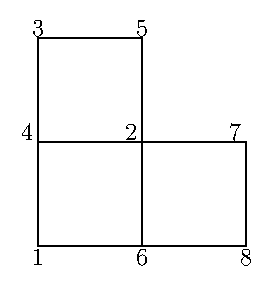
\includegraphics[scale=1]{Figs/genmap_sketch}
\caption{Two-dimensional mesh}
\label{fig:genmap}
\end{figure}

Let us a regard the mesh in Fig.~\ref{fig:genmap} as a graph of \(N\) vertices and \(M\) edges, \(G(V_N,E_M)\). We define the Laplacian matrix associated to a graph \(G\) as \(L(G)\). We define as the degree of a node \(V_i\) the number of incident edges, e.g. in Fig.~\ref{fig:genmap} \(deg(V_2)=4\) and \(deg(V_6)=3\).
\begin{equation}
L(G)_{ij}= \left\{
  \begin{array}{l l}
    i=j & \quad \mathrm deg(V_i)\\
    i\neq j & \quad -1 \text{ if there is and edge (i,j) and } 0 \text{ otherwise}
  \end{array} \right .
\end{equation}

\begin{equation}
L(G)= \begin{pmatrix} 
  &1 & 2 & 3 & 4 & 5 & 6 & 7 & 8\\ 
  \hline
1| &2 & 0 & 0 & -1 & 0 & -1 & 0 & 0\\ 
2| &0 & 4 & 0 & -1 & -1 & -1 & -1 & 0\\  
3| &0 & 0 & 2 & -1 & -1 & 0 & 0 & 0\\ 
4| &-1 & -1 & -1 & 3 & 0 & 0 & 0 & 0\\ 
5| &0 & -1 & -1 & 0 & 2 & 0 & 0 & 0\\ 
6| &-1 & -1 & 0 & 0 & 0 & 3 & 0 & -1\\ 
7| &0 & -1 & 0 & 0 & 0 & 0 & 2 & -1\\ 
8| &0 & 0 & 0 & 0 & 0 & -1 & -1 & 2\\  
\end{pmatrix}
\end{equation}

Properties of \(L(G)\)
\begin{itemize}
\item \(L(G)\) symmetric
\item the unit vector \(e=[1, \ldots 1]\in \mathcal{N}(L(G))\) is in the nullspace of the Laplacian matrix
\item \(\forall\lambda \in \sigma(L(G)>0\), i.e. all the eigenvalues of \(L(G)\) are positive except \(\lambda_0\) corresponding to the unit vector
\item \(\lambda_2\neq 0\) if the graph is connected, \(\lambda_2(L(G))\) is also called the algebraic connectivity of the graph
\end{itemize}

The main ides of the spectral bisection algorithm is
\begin{verbatim}
compute \(v_2\) eigenvector corresponding to \(\lambda_2(L(G))\)
for i=1,N
  if v_2(i) < 0 put vertex \(V_i\) in N_{-} 
  else put vertex \(V_i\) in N_{-} 
\end{verbatim}

The eigenvectors and eigenvalues are computed using Lanczos's algorithm.
These steps are repeated recursively on each of the two branches of the graph \(N_{-}, N_{+}\). This is possible since according to Fiedler's theorems the graph \(N_{-}\) is connected, \(N_{+}\) connected only if no \(v_2(i)=0\),  and for each subgraph \(G_1\) the algebraic connectivities satisfy \(\lambda_2(L(G_1))\leq\lambda_2(L(G))\).



To run the genmap code be sure that the Nek tools are up-to-date and compiled. 
At command line type: genmap 
NOTE-If the executables for the tools were not placed in the bin directory(default), 
include the path to the genmap executable. We give here the output for the .rea file in the Kovasznay example
\begin{verbatim}
Input (.rea) file name:
kov
Input mesh tolerance (default 0.2):
NOTE: smaller is better, but generous is more forgiving for bad meshes.
0.05
 reading .rea file data ...
 start locglob_lexico:           8         960        7680  0.10000000000000001     
 locglob:           1           1        7680
 .....
 locglob:           3        1254        7680
 done locglob_lexico:        1254        1254        7680           8
 start periodic vtx:         960        1254
 done periodic vtx
 start rec_bisect:         960
 done:    0.1% 
 .....
 done:   99.4% 
  
 done rec_bisect
writing kov.map    
\end{verbatim}
The user is prompted for .rea file name and should enter only the prefix of the .rea file. 
The user is prompted for mesh tolerance value. Typically a value of .05 is sufficient. Increasing or decreasing this value should make very little difference in the mesh generation. However, if given an error from genmap, the tolerance may need to be made slightly more generous. 

A successful genmap run will produce a .map file with the proper processor decomposition.


NOTE: For large element counts, it is not uncommon for genmap to be produce a few disconnected sets.  
These sets are typically under 7 elements large and  will not affect optimization of the NEK5000 run.  
If a disconnected set is produced, genmap will output the following warning to stdout.
\begin{verbatim}
 not connected   N0   NEL  Nsets   Nlarge sets
\end{verbatim}  
Here, {\tt N0} is the number of elements disconnected from the set of {\tt NEL} elements, {\tt Nsets} is the counter of disconnected sets found, 
and {\tt Nlarge sets} is the number of sets greater than 64 elements in size.  {\tt Nlarge sets} should always be 0.  If not, please contact someone on the developer team so we can be sure to have a more optimal partition of your mesh.

Genmap outputs an ordered set of numbers which are organized as follows
Line number 1 contains the header {\tt nel, nactive, depth, d2, npts, nrank, noutflow}

\begin{itemize}
\item {\tt nel}  number of elements
\item {\tt nactive} nrank-noutflow
\item {\tt depth} floor(log2(nel))
\item {\tt d2} \(2^{depth}\)
\item {\tt npts} number of corner points ({\tt nel*4} in 2D, {\tt nel*8} in 3D)
\item {\tt nrank} number of unique corner points
\item {\tt noutflow} number of outflows (not used anymore, is zero)
\end{itemize}

For the Kovasnay flow on an 8 element mesh with periodic boundary conditions we have
 {\tt 8         12          3          8         32         12          0}
 

Next we have the data (one line per element, listed in order of global element number)
====
{\tt 6          12          11           6           5}

This means that elemnt one (since we are on the first line) belongs to group 6, and this element is given by vertices in unique ordering. 
The vertices are ordered in symmetric ordering (starting at 1)

3 - 4
|   |
1 - 2

To distribute amongst processors, one just takes as many consecutive
processors as one wants.
